\section{Signal Model}
\label{sec:model}

\begin{figure*}[t]
  \centerline{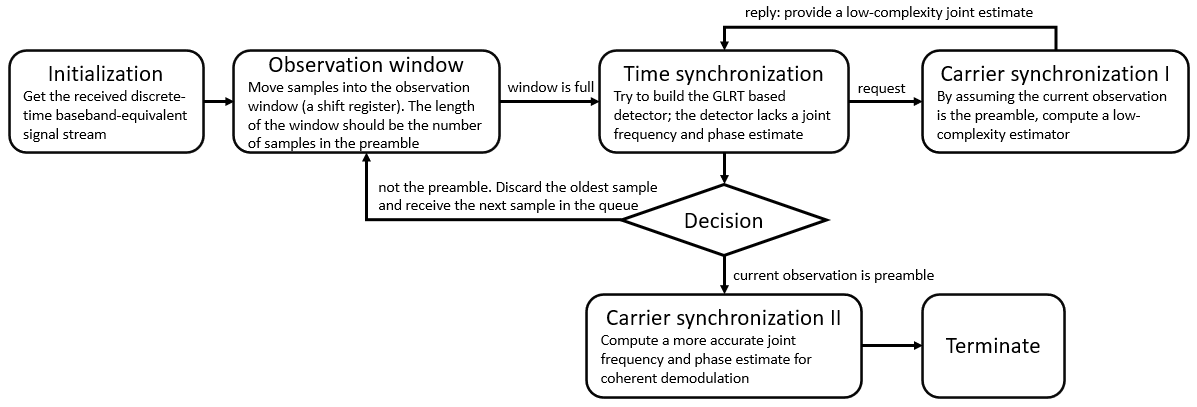
\includegraphics[width=6.5in]{signal_acquisition_chain.png}}
  \caption{Block diagram for analysis of the complete signal acquistion chain}
  \label{fig:sig_acquis_chain}
  \end{figure*}

The transmitted signal burst is assumed to include a refere\-nce signal that is known to the receiver.
Often such a reference sequence is prepended to the payload and is referred to as a preamble.
The problem addressed in this paper is to accurately estimate the start time of the preamble and 
to estimate carrier phase and frequency offset from this preamble.
Hence, the payload portion of the burst is not further considered.

The baseband-equivalent reference signal $s(t)$ is digitally modulated as
\begin{equation}
    \label{eq:l_ref_sig_analog}
    s(t) = \sum_{i=0}^{L_0-1} c_i g(t-iT),
  \end{equation}
where $T$ denotes the symbol period and $g(t)$ provides pulse shaping. $c_i$ are the known symbol sequence
between transmitter and receiver, and $L_0$ is the number of symbols. It is common to assume the symbols 
$\{c_i\}$ have good autocorrelation properties to render coherent processing effective.

The received baseband equivalent signal stream are given by
\begin{equation}
    \label{eq:rec_sig_analog}
    r(t) = s(t-\tau) \cdot Ae^{j \phi} e^{j2\pi f_d t} + w(t).
  \end{equation}
where $\tau$ denotes the delay (the start time) of received reference signal in stream. $A$, $\phi$, $f_d$ 
are the carrier amplitude, phase, and frequency offset, respectively. These are the parameters to be estimated
for signal acquisition. The complex, additive white Gaussian noise is denoted $w(t)$.

Our algorithms operate in discrete-time; sampling the received signal $r(t)$ at a rate of $M$ samples per symbol,
i.e., the sampling frequency $f_s=\frac{1}{T_s}=\frac{M}{T}$, yields 
\begin{equation}
    \begin{aligned}
      \label{eq:model}
      r_n = s_{n-p}Ae^{j\phi}e^{j2\pi\delta n}+w_{n},
    \end{aligned}
  \end{equation}
The continuous-time delay $\tau$ is decomposed into $\tau=pT_s+\Delta p$ with $pTs$ integer multiples of sample period and 
the fractional delay $\Delta p$ satisfying $-Ts/2 < \Delta p \leq T_s/2$. $\Delta p$ is neglected in this paper because 
our proposed algorithm proceeds at a very sufficient sample rate (in SDR). $\delta=f_d T_s$ is the normalized frequency offset. 
Besides that, we use $E_s/N_0$ to represent the ratio of signal energy to noise power spectral density (SNR).
Specifically, $E_s$ is the averaged symbol energy of the received signal over the length of the preamble.

% estension to reviewer 3, comment 3
Our goal of this paper is to analyze the complete signa\-l acquisition chain, which includes
the detection (time synchronization) and joint phase and frequency estimation of the preamble (carrier synchronization). 
The procedure is depicted in Figure~\ref{fig:sig_acquis_chain}.
The analysis of the signal acquisition chain will basically follow the steps 
that are shown in the figure as well as be implemented in software-defined radio (SDR).